\documentclass[12pt,b5paper]{ltjsarticle}

%\usepackage[margin=15truemm, top=5truemm, bottom=5truemm]{geometry}
\usepackage[margin=15truemm]{geometry}

\usepackage{amsmath,amssymb}
%\pagestyle{headings}
\pagestyle{empty}

%\usepackage{listings,url}
%\renewcommand{\theenumi}{(\arabic{enumi})}

\usepackage{graphicx}

\usepackage{tikz}
\usetikzlibrary {arrows.meta}
\usepackage{wrapfig}	% required for `\wrapfigure' (yatex added)
\usepackage{bm}	% required for `\bm' (yatex added)
\usepackage{luatexja-ruby}	% required for `\ruby'
%% 像Im を定義
%\newcommand{\Img}{\mathop{\mathrm{Im}}\nolimits}

\usepackage{multicol}	% required for `\multicols' (yatex added)
\begin{document}



\hrulefill
\begin{multicols}{2}
 \begin{enumerate}
  \item $3.8^0$
  \item $9^{0.5}$
  \item $10^{-5}$ (小数表記)
  \item $16^{\frac{3}{2}}$
  \item $5^3 \times 5^{-2.8}$
  \item $3^3 \div 3^{\frac{6}{5}}$
  \item $\left(2^{-\frac{2}{3}}\right)^{-\frac{9}{2}}$
  \item $\displaystyle \frac{a^{\frac{1}{3}}\times a^{\frac{2}{3}}}{a^{\frac{9}{4}}}$
  \item $\left( a^{\frac{1}{2}} - b^{\frac{1}{2}} \right)^2$
 \end{enumerate}
\end{multicols}

\dotfill

\textbf{指数法則}
\begin{multicols}{2}
$a^b$について
\begin{itemize}
 \item $a=0$の時、$a^b = 0$
 \item $b=0$の時、$a^b = 1$
 \item $a=0, b=0$の時、$a^b$は定義できない
\end{itemize}

$a\ne 0, n\ne 0, m\ne 0$とする。
\begin{itemize}
 \item $a^n=\frac{1}{a^{-n}}$
 \item $a^n \times a^m = a^{n+m}$
 \item $(a^n)^m = a^{nm}$
 \item $a^{\frac{n}{m}} = \sqrt[m]{a^n}$
\end{itemize}
\end{multicols}

\dotfill

 \begin{enumerate}
  \item $3.8^0$ $=1$
  \item $9^{0.5}$ $=(3^2)^{0.5}=3^{2 \times 0.5} =3$
  \item $10^{-5}$ $=\frac{1}{10^5}=0.00001$
  \item $16^{\frac{3}{2}}$ $=(2^4)^{\frac{3}{2}} = 2^6 = 64$
  \item $5^3 \times 5^{-2.8}$ $=5^{3-2.8}=5^{0.2} =\sqrt[5]{5}$
  \item $3^3 \div 3^{\frac{6}{5}}$ $=3^{3-\frac{6}{5}}=3^{\frac{9}{5}} =\sqrt[5]{3^9}$
  \item $\left(2^{-\frac{2}{3}}\right)^{-\frac{9}{2}}$
        $=2^{{-\frac{2}{3}} \times (-\frac{9}{2})}=2^3=8$
  \item $\displaystyle \frac{a^{\frac{1}{3}}\times a^{\frac{2}{3}}}{a^{\frac{9}{4}}}$
        $= a^{ \frac{1}{3} + \frac{2}{3} - \frac{9}{4} } = a^{-\frac{5}{4}} = \frac{1}{\sqrt[4]{a^5}}$
  \item $\left( a^{\frac{1}{2}} - b^{\frac{1}{2}} \right)^2$
        $= (a^{\frac{1}{2}})^2 -2a^{\frac{1}{2}} b^{\frac{1}{2}} + (b^{\frac{1}{2}})^2 = a-2\sqrt{ab} + b$
 \end{enumerate}


\hrulefill

$\theta = 30^{\circ}$の傾斜上で、物体が初速度$v_0 = 15_\mathrm{[m/s]}$ で上方に発射された。
物体と斜面間の摩擦係数は$\mu = 0.2$とし、
物体が到達する最高地点までの距離$x_\mathrm{[m]}$及び
要する時間 $t_\mathrm{[s]}$を求めよ。

\begin{center}
 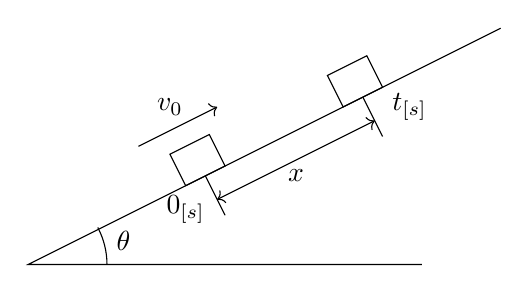
\begin{tikzpicture}
  \draw (5,0)--(0,0)--(6,3);
  \draw (1,0) arc (0:28:1);
  \node at (1,0.3) [right] {$\theta$};

  \draw (2,1)--(1.8,1.4)--(2.3,1.65)--(2.5,1.25)--cycle;
  \draw[->] (1.4,1.5)--(2.4,2);
  \node at (1.8,2) {$v_0$};

  \draw (4,2)--(3.8,2.4)--(4.3,2.65)--(4.5,2.25)--cycle;

  \draw (2.25,1.125)--(2.5,0.625);
  \draw (4.25,2.125)--(4.5,1.625);
  \draw[<->] (2.4,0.825)--(4.4,1.825);
  \node at (2,1) [below] {$0_{[s]}$};
  \node at (4.5,2) [right] {$t_{[s]}$};
  \node at (3.4,1.325) [below] {$x$};
 \end{tikzpicture}
\end{center}


物体の質量を$m$、重力加速度を$g$とする。

物体に働く重力は$mg$である。
これを斜面に対して平行と垂直な成分に分ける。
\begin{itemize}
 \item 平行な向き $mg \sin 30^{\circ} = mg/2$
 \item 垂直な向き $mg \cos 30^{\circ} = \sqrt{3}mg/2$
\end{itemize}

摩擦力は垂直抗力を$N$とすると$\mu N$であるので、
\begin{equation}
 \mu N = \mu mg \cos 30^{\circ} = \sqrt{3}mg/10
\end{equation}
である。

斜面方向の物体にかかる力は
斜面方向の重力と摩擦力である。
斜面を移動する物体の加速度を$a$とすると次の式が出来る。
\begin{equation}
 ma = -mg \sin 30^{\circ} - \mu mg \cos 30^{\circ}
\end{equation}
ここから物体の加速度$a$が求まる。
\begin{equation}
 a = -g \left( \sin 30^{\circ} + \mu \cos 30^{\circ}\right)
\end{equation}

物体の速度$v$を求める為、加速度$a$を時間$t$で積分する。
\begin{equation}
 v = -g ( \sin 30^{\circ} + \mu \cos 30^{\circ} )t +C
\end{equation}
速度は初速が$v_0$であるので、
$(t,v)=(0,v_0)$を代入すると$C=v_0$となる。
つまり、$v$の式は次のようになる。
\begin{equation}
 v = -g ( \sin 30^{\circ} + \mu \cos 30^{\circ} )t + v_0
  \label{v}
\end{equation}


距離$x$を求める為、速度$v$を時間$t$で積分する。
\begin{equation}
 x = -\frac{1}{2}g ( \sin 30^{\circ} + \mu \cos 30^{\circ} )t^2 + v_0t + C
\end{equation}
時間$t=0$の時、距離$x=0$であるのでこれを代入すると$C=0$である。
これにより距離$x$の式は次のようになる。
\begin{equation}
 x = -\frac{1}{2}g ( \sin 30^{\circ} + \mu \cos 30^{\circ} )t^2 + v_0t
  \label{x}
\end{equation}

最高地点に到達する時間を$t_1$とすると、
その時の物体の速さは$0$である。
この為、式(\ref{v})に$(t,v)=(t_1,0)$を代入する。
\begin{align}
 0 = -g ( \sin 30^{\circ} + \mu \cos 30^{\circ} )t_1 + v_0\\
 t_1 = \frac{v_0}{g ( \sin 30^{\circ} + \mu \cos 30^{\circ} )}\label{at}
\end{align}

この時間$t=t_1$を距離$x$の式(\ref{x})に代入する。
\begin{align}
 x =& -\frac{1}{2}g ( \sin 30^{\circ} + \mu \cos 30^{\circ} )\left(\frac{v_0}{g ( \sin 30^{\circ} + \mu \cos 30^{\circ} )}\right)^2 + v_0\left(\frac{v_0}{g ( \sin 30^{\circ} + \mu \cos 30^{\circ} )}\right)\\
 =& -\frac{v_0^2}{2g( \sin 30^{\circ} + \mu \cos 30^{\circ} )}
 + \frac{v_0^2}{g ( \sin 30^{\circ} + \mu \cos 30^{\circ} )}\\
 =& \frac{v_0^2}{2g ( \sin 30^{\circ} + \mu \cos 30^{\circ} )}\label{ax}
\end{align}

式(\ref{at})と式(\ref{ax})に
$(v_0,\mu)=(15, 0.2)$を代入すると
\begin{align}
 t_1 =& \frac{v_0}{g ( \sin 30^{\circ} + \mu \cos 30^{\circ} )}
 = \frac{15}{g ( \frac{1}{2} + 0.2 \times \frac{\sqrt{3}}{2} )}\\
 =& \frac{150}{g(5+\sqrt{3})}
 = \frac{75}{11g}(5-\sqrt{3})\\
%
 x =& \frac{v_0^2}{2g ( \sin 30^{\circ} + \mu \cos 30^{\circ} )}
 = \frac{15^2}{2g ( \frac{1}{2} + 0.2 \times \frac{\sqrt{3}}{2} )}\\
 =& \frac{15^2 \times 5}{g ( 5+\sqrt{3} )}
 = \frac{1125}{22g} ( 5-\sqrt{3} )
\end{align}
である。

よって、
最高地点までの距離は
\begin{equation}
 \frac{1125}{22g} ( 5-\sqrt{3} )
\end{equation}
要する時間は
\begin{equation}
 \frac{75}{11g}(5-\sqrt{3})
\end{equation}
である。




\end{document}
